\section{Limpieza de datos}\label{sec:limpieza}

Cada fuente se limpia con su propio script en \archivo{src/clean/}. Todos leen de
\archivo{data/raw/} sin modificar los originales y escriben en \archivo{data/interim/} en dos
formatos: CSV, el principal, que se abre en Excel y en cualquier programa, y Parquet, un respaldo más
ligero que conserva los tipos de dato. La base de carpetas de la FGJ tiene 1.9 millones de filas, más de
las 1,048,576 que admite Excel, por lo que se trabaja con pandas o con su versión agregada. Cada script genera además un reporte en \archivo{docs/limpieza_<fuente>.md}, con el número
de registros afectados en cada paso.

\subsection{Catálogos comunes}
El módulo \archivo{catalogos.py} concentra lo que comparten todas las fuentes:
\begin{itemize}
  \item \textbf{Catálogo de alcaldías.} Las 16 alcaldías con su clave INEGI (\archivo{09002} a
        \archivo{09017}) y sus polígonos, leídos directamente del Marco Geoestadístico 2020.
  \item \textbf{Normalización de texto.} Repara el \emph{mojibake}, quita acentos, pasa a
        mayúsculas y elimina espacios repetidos. Así \enquote{Álvaro Obregón}, \enquote{ALVARO OBREGON}
        y su versión mal codificada se reconocen como la misma alcaldía.
  \item \textbf{Asignación por coordenadas.} Ubica la alcaldía de un punto (latitud, longitud)
        mediante una prueba de punto en polígono.
\end{itemize}

\subsection{Carpetas de investigación (FGJ)}

\paragraph{Decisiones principales.}
\begin{enumerate}
  \item \textbf{Fecha del hecho, no de inicio.} Cada archivo anual contiene las carpetas
        \emph{iniciadas} ese año, que pueden referirse a hechos anteriores. Para medir cuándo ocurren
        los delitos se usa \archivo{fecha_hecho}. La mediana del retraso entre el hecho y la denuncia
        es de 1 día, pero el percentil 90 es de 56 días.
  \item \textbf{Ventana 2016 -- julio de 2024.} Se descartan los hechos anteriores a 2016: solo
        aparecen si se denunciaron desde 2016, así que su registro está incompleto. Por la misma razón,
        junio y julio de 2024 se marcan como \emph{meses incompletos}, porque todavía faltan las
        denuncias tardías.
  \item \textbf{Alcaldía.} Se toma de \archivo{alcaldia_hecho}. Coincide con la alcaldía calculada por
        coordenadas en el 99.7\,\% de los casos. Los registros \enquote{CDMX (indeterminada)} no
        traen coordenadas, así que se conservan para el total de la ciudad con la clave \archivo{09000}.
  \item \textbf{Duplicados.} El archivo no trae un identificador de carpeta. Las 3,824 filas
        idénticas en las 21 columnas (0.19\,\%) tienen como hora de inicio \archivo{00:00:00}, un valor de relleno, y son sobre todo fraude y
        abuso de confianza, lo que sugiere denuncias múltiples de un mismo hecho. Se \emph{marcan} en
        lugar de borrarse, y el conteo agregado las excluye.
  \item \textbf{Grupos de delito estables.} Los 352 delitos distintos se agrupan en 22 categorías
        mediante palabras clave, no por nombre exacto. Así, los cambios de denominación del catálogo
        de 2019 (nota de reclasificación de la FGJ) no rompen las series. Solo el 7\,\% queda en
        \enquote{otros}, y las 16 categorías de alto impacto de la FGJ caen cada una en un único grupo.
\end{enumerate}

\begin{table}[h]
\centering
\caption{Pasos de limpieza de las carpetas de la FGJ.}\label{tab:limpieza_fgj}
\small
\begin{tabular}{lrl}
\toprule
\textbf{Paso} & \textbf{Registros} & \textbf{Acción}\\
\midrule
Registros leídos (9 archivos) & 1,987,424 & ---\\
Idénticos en las 21 columnas & 3,824 & se marcan\\
Sin fecha del hecho & 545 & se descartan\\
Hecho anterior a 2016 & 32,223 & se descartan\\
Hecho posterior al inicio de la carpeta & 110 & se descartan\\
Hecho fuera de la CDMX & 16,734 & se descartan\\
En la CDMX sin alcaldía identificable & 18,595 & se conservan (clave 09000)\\
Hechos no delictivos & 66,960 & se marcan\\
Últimos 2 meses (subregistro) & 30,814 & se marcan\\
\midrule
\textbf{Base limpia} & \textbf{1,937,812} & 97.5\,\% del original\\
\bottomrule
\end{tabular}
\end{table}

\paragraph{Salidas.} \archivo{fgj_carpetas.parquet}, con una fila por carpeta, y
\archivo{fgj_alcaldia_mes.parquet}, con los conteos por alcaldía, mes y grupo de delito
(34,683 filas). Esta tabla incluye la clave INEGI y el nombre de la alcaldía; las carpetas sin
alcaldía identificable aparecen con la clave 09000 y el nombre \enquote{CDMX (sin alcaldía)}.

\paragraph{Primeros resultados.} La Figura~\ref{fig:fgj_grupos} muestra tres grupos con
comportamientos distintos:
\begin{itemize}
  \item \textbf{Robo a transeúnte:} cayó con el confinamiento y no se ha recuperado (18,528
        carpetas en 2019, 12,306 en 2020 y 10,682 en 2023). Sin embargo, \emph{ya venía bajando
        desde finales de 2018}, así que no toda la caída puede atribuirse a la pandemia.
  \item \textbf{Violencia familiar:} bajó en abril de 2020, probablemente porque el confinamiento
        dificultó denunciar, y después subió con fuerza (25,802 en 2019, 28,340 en 2020 y 37,310
        en 2023). Esto es consistente con la hipótesis H2.
  \item \textbf{Robo en transporte público:} cayó a menos de la mitad y se estabilizó en ese nivel,
        igual que la afluencia del Metro.
\end{itemize}

\begin{figure}[h]
\centering
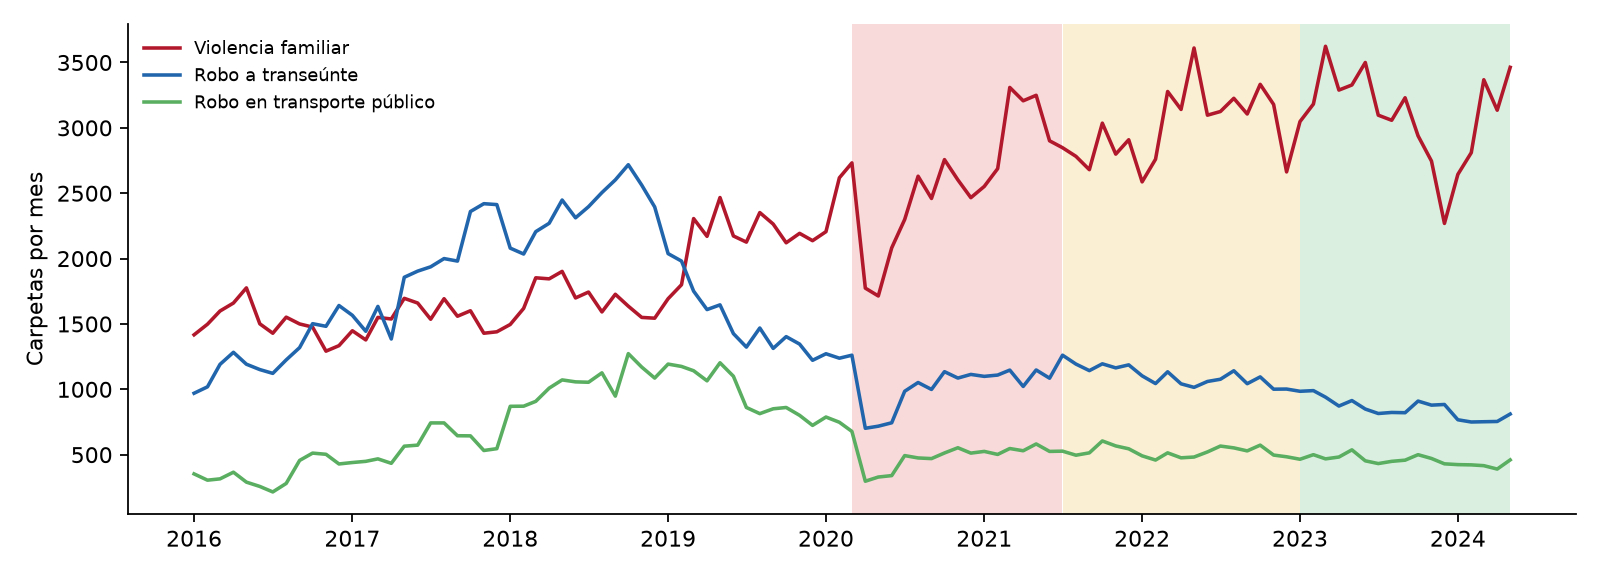
\includegraphics[width=\textwidth]{figuras/fgj_grupos_mes.png}
\caption{Carpetas mensuales por grupo de delito (sin los meses incompletos). Fuente: elaboración
propia con datos de la FGJ.}\label{fig:fgj_grupos}
\end{figure}

\subsection{Afluencia del Metrobús}

\begin{table}[h]
\centering
\caption{Pasos de limpieza del Metrobús.}\label{tab:limpieza_mb}
\small
\begin{tabular}{L{8.5cm}L{5.5cm}}
\toprule
\textbf{Paso} & \textbf{Resultado}\\
\midrule
Registros leídos (fecha × línea) & 53,732\\
Nombres de línea (\archivo{Línea N} / \archivo{linea N} en 2023) & 14 $\rightarrow$ 7 unificados\\
Vacíos antes de la inauguración de cada línea & 17,227; no son faltantes, se marcan\\
Faltantes con la línea operando & 0\\
Duplicados fecha × línea & 0\\
Días atípicos respecto a la mediana móvil de 29 días & 30; se conservan (eventos reales)\\
Errores evidentes & 2; se anulan\\
Valores con decimales (Línea~4, ene--feb 2025) & 57; se redondean y se marcan como estimados\\
\bottomrule
\end{tabular}
\end{table}

\paragraph{Valores atípicos.} Se compararon con la mediana móvil de 29 días de la misma línea.
Casi todos los días bajos corresponden a hechos reales: domingos, 1 de enero, el día posterior al
sismo del 19-S de 2017, la jornada electoral de 2018, la visita papal de 2016 y los desfiles del 16
de septiembre. Esos se conservan. Solo se anularon dos errores evidentes:
\begin{itemize}
  \item 26 de julio de 2005, Línea~1: 3.03 millones de viajes, unas 13 veces un día normal.
        Probablemente es el acumulado desde la inauguración.
  \item 20 de septiembre de 2017, Línea~2: 9 pasajeros.
\end{itemize}

\paragraph{Metro frente a Metrobús.} Ambos sistemas cayeron casi lo mismo en mayo de 2020: el Metro
a un índice de 26.5 y el Metrobús a 24.2, con 2019 = 100. Sin embargo, su recuperación fue muy
distinta (Figura~\ref{fig:metro_mb}). El Metrobús superó su nivel de 2019 a partir de la segunda mitad
de 2022 y en 2024 alcanzó un promedio anual de 118.9. El Metro, en cambio, se ha quedado entre 73 y 79
(promedios anuales de 2024 y 2025). Esto puede deberse a la ampliación de la
red del Metrobús y al traslado de usuarios por los cierres de las Líneas~1 y 12 del Metro. Es una
pregunta que conviene responder en la fase de análisis.

\begin{figure}[h]
\centering
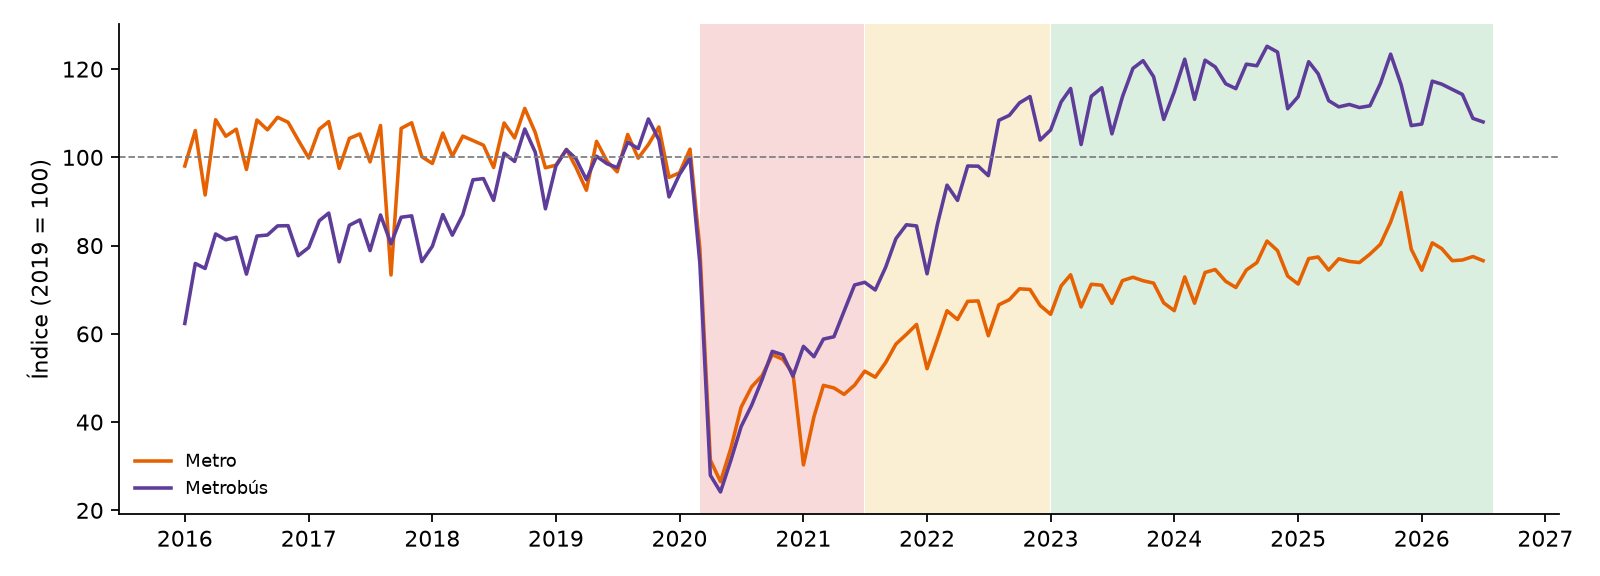
\includegraphics[width=\textwidth]{figuras/metro_vs_metrobus.png}
\caption{Afluencia diaria promedio mensual del Metro y del Metrobús, índice 2019 = 100. Fuente:
elaboración propia con datos del STC Metro y del Metrobús.}\label{fig:metro_mb}
\end{figure}

\subsection{Puestos de trabajo asegurados (IMSS)}
La limpieza del IMSS se hizo paso a paso en el notebook \archivo{01_limpieza_datasets.ipynb}. El
resultado, \archivo{imss_subdelegacion_mes.csv}, tiene una fila por mes y subdelegación del IMSS:
128 meses por 10 subdelegaciones, es decir, 1,280 filas.

\paragraph{Decisiones.}
\begin{itemize}
  \item \textbf{Medida de empleo:} se usan los \emph{puestos de trabajo} (\archivo{ta}) y no los
        \emph{asegurados}, que incluyen a personas afiliadas sin empleo. En la CDMX hay unos 5
        millones de asegurados, pero solo unos 3.5 millones de puestos.
  \item \textbf{Territorio:} el IMSS no publica la CDMX por alcaldía. Las delegaciones (Norte y Sur)
        y las subdelegaciones son oficinas del IMSS, y los empleos se registran donde la empresa dio
        de alta su registro patronal. Por eso solo se usan como dato complementario.
  \item \textbf{Columnas cambiantes:} el IMSS agregó \archivo{rango_uma} en febrero de 2017 y
        \archivo{ptpd} en 2026, y en 7 meses publicó un nombre de columna mal codificado. El código
        lee solo las columnas necesarias, con el nombre que tengan en cada archivo.
  \item \textbf{Vacíos en el rango salarial:} el 99.7\,\% corresponde a asegurados sin empleo, que no
        tienen salario, así que no se imputan. Los puestos sin rango (menos del 0.5\,\%) van a una
        categoría \enquote{sin dato}.
  \item \textbf{Rango de UMA en 2016:} se copió el rango en salarios mínimos, porque en 2016 la UMA
        valía lo mismo que el salario mínimo (\$73.04). Enero de 2017 queda aproximado.
\end{itemize}

\paragraph{Validación.} No faltan meses. Hombres, mujeres y no binario suman exactamente los
puestos, y los rangos salariales también. Diciembre de 2019 coincide con la cifra calculada
directamente del archivo original (3,470,048 puestos).

\begin{table}[h]
\centering
\caption{Puestos de trabajo formales en la CDMX (IMSS).}\label{tab:imss}
\small
\begin{tabular}{lrrr}
\toprule
\textbf{Mes} & \textbf{Puestos} & \textbf{Mujeres} & \textbf{Salario diario (nominal)}\\
\midrule
Diciembre 2019 & 3,470,048 & 1,447,069 & \$471\\
Diciembre 2020 & 3,246,669 & 1,347,572 & \$510\\
Marzo 2021 (mínimo) & 3,213,626 & 1,338,652 & \$539\\
Diciembre 2024 & 3,479,354 & 1,518,611 & \$729\\
Agosto 2026 & 3,689,815 & 1,585,251 & \$801\\
\bottomrule
\end{tabular}
\end{table}

\paragraph{Primeros resultados.} Entre febrero y diciembre de 2020 se perdieron unos 200 mil
empleos formales, y el punto más bajo llegó en marzo de 2021, con unos 233 mil puestos menos que en
febrero de 2020. El promedio anual volvió a 99.6 (2019 = 100) en 2023 y a 101.2 en 2024. El
empleo formal se recuperó mucho antes que la afluencia del Metro, que sigue entre 73 y 79, lo cual
apoya la hipótesis H3.

\paragraph{Advertencia sobre los rangos salariales.} El grupo \enquote{hasta 2 UMA} pasa de
1.17~millones de puestos en 2019 a 21~mil en 2024. No es un error: el salario mínimo subió hasta
equivaler a unas 2.3 UMA, así que ya nadie puede ganar legalmente menos de 2 UMA. Por eso, para
comparar salarios antes y después de la pandemia se usará el salario promedio \emph{deflactado}
con el INPC. El salario nominal subió 55\,\% entre 2019 y 2024, con una inflación cercana al 30\,\%.

\paragraph{Gráficas.} La Figura~\ref{fig:imss_top} muestra las cinco subdelegaciones con más empleo
formal. Polanco concentra cerca de 700 mil puestos porque ahí registran su plantilla muchas empresas
grandes, no porque ahí trabaje toda esa gente. Desde finales de 2025, San Ángel presenta saltos de
hasta $\pm$60 mil puestos de un mes a otro, que no aparecen en el total de la ciudad. Probablemente se
deben a reasignaciones administrativas de registros patronales entre subdelegaciones, así que no deben
interpretarse como cambios de empleo.

\begin{figure}[h]
\centering
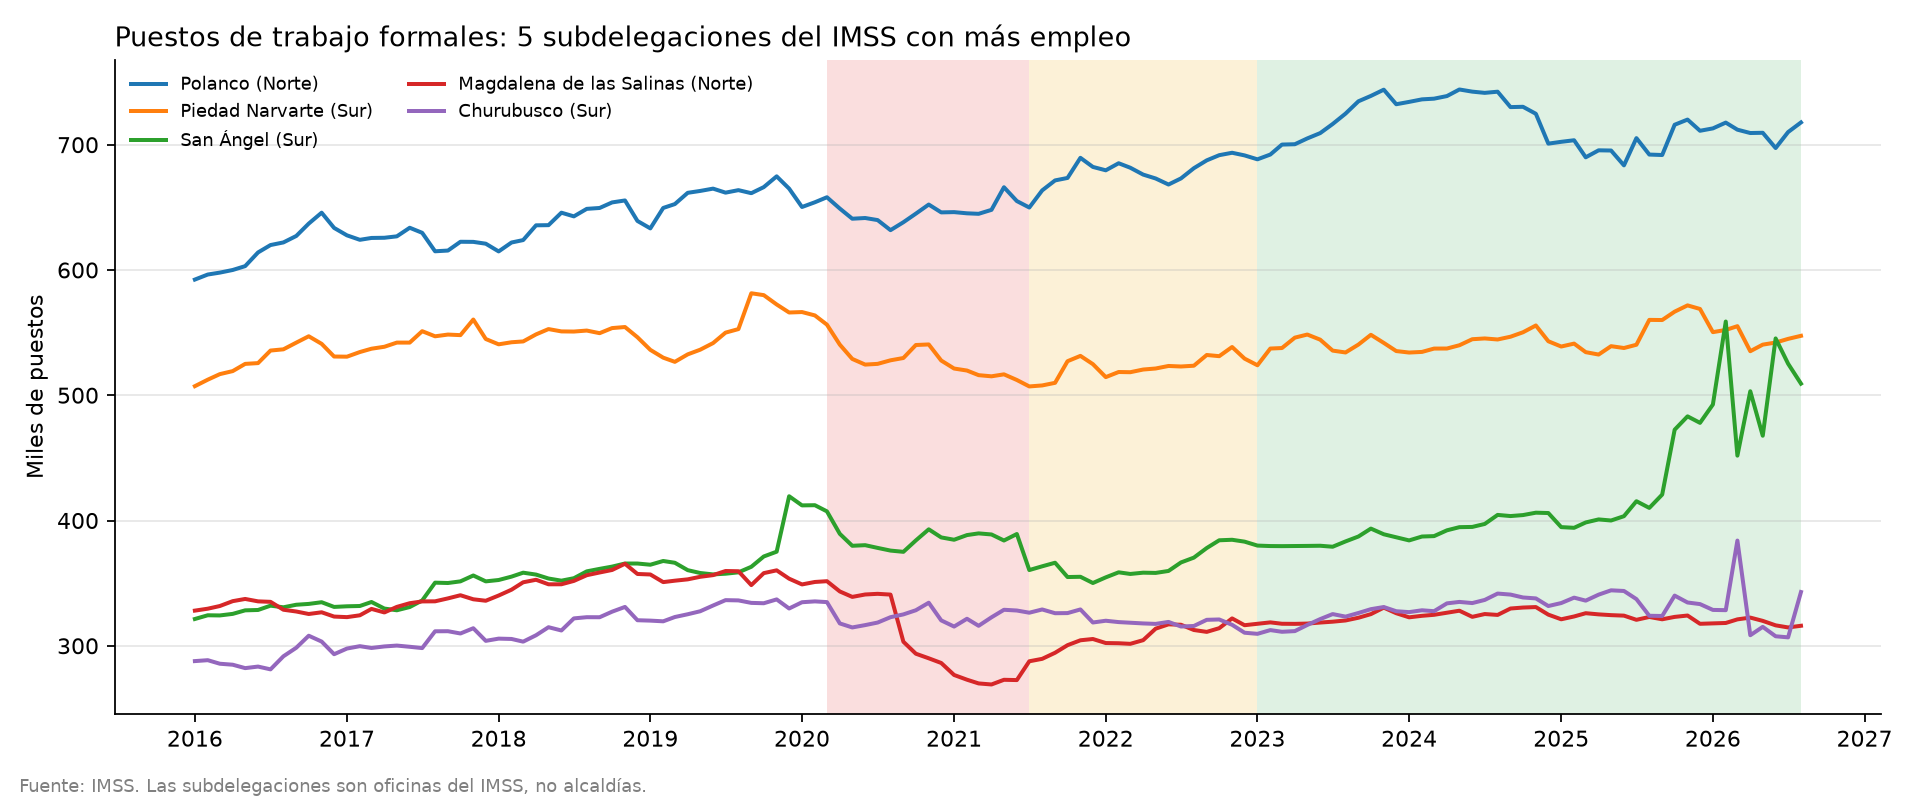
\includegraphics[width=\textwidth]{figuras/imss_top_subdelegaciones.png}
\caption{Puestos de trabajo formales en las cinco subdelegaciones del IMSS con más empleo en 2019.}\label{fig:imss_top}
\end{figure}

La Figura~\ref{fig:imss_rangos} muestra la distribución por rango salarial. Hay dos caídas abruptas
del grupo \enquote{hasta 2 UMA}, en enero de 2022 (a 0.3\,\%, y en febrero regresa a 22\,\%) y en
enero de 2023 (definitiva). Se explican por el calendario: el salario mínimo sube el 1 de enero y la
UMA hasta el 1 de febrero. En enero de 2022, el salario mínimo integrado ($\approx$\$180.7) quedó
apenas por encima de 2 UMA de 2021 (\$179.24); en febrero, con la UMA nueva, volvió a quedar por
debajo. Desde 2023 el mínimo supera las 2 UMA de forma permanente. Es un efecto de la política
salarial y no un error de los datos.

\begin{figure}[h]
\centering
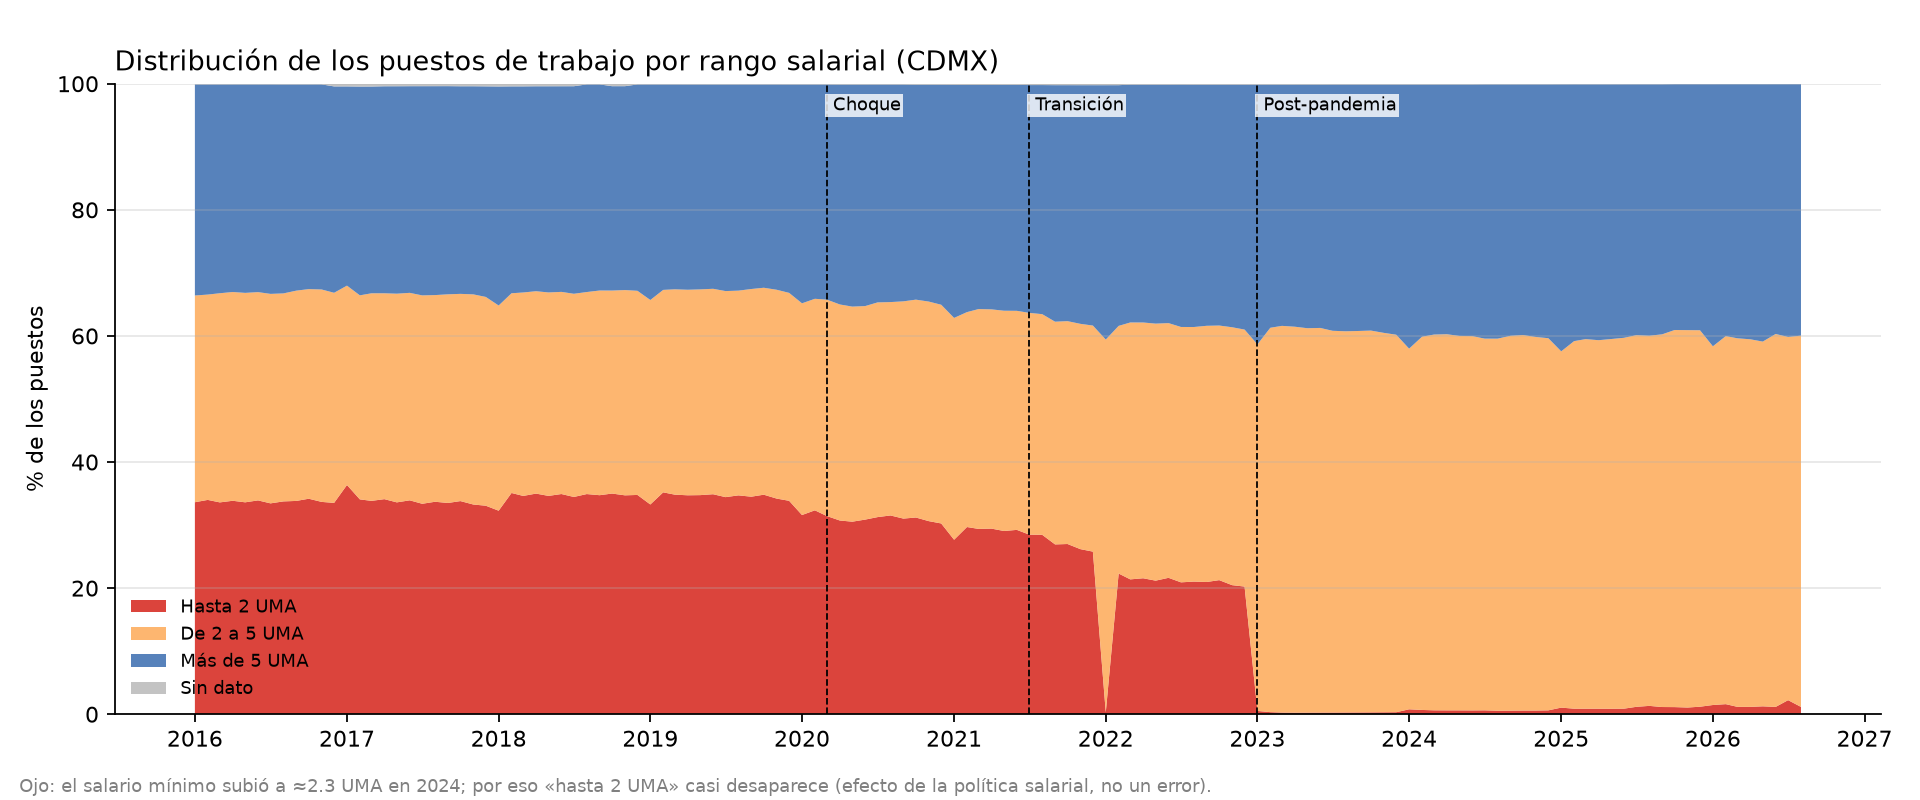
\includegraphics[width=\textwidth]{figuras/imss_rangos_uma.png}
\caption{Distribución de los puestos de trabajo por rango salarial en UMA, CDMX.}\label{fig:imss_rangos}
\end{figure}

\begin{figure}[h]
\centering
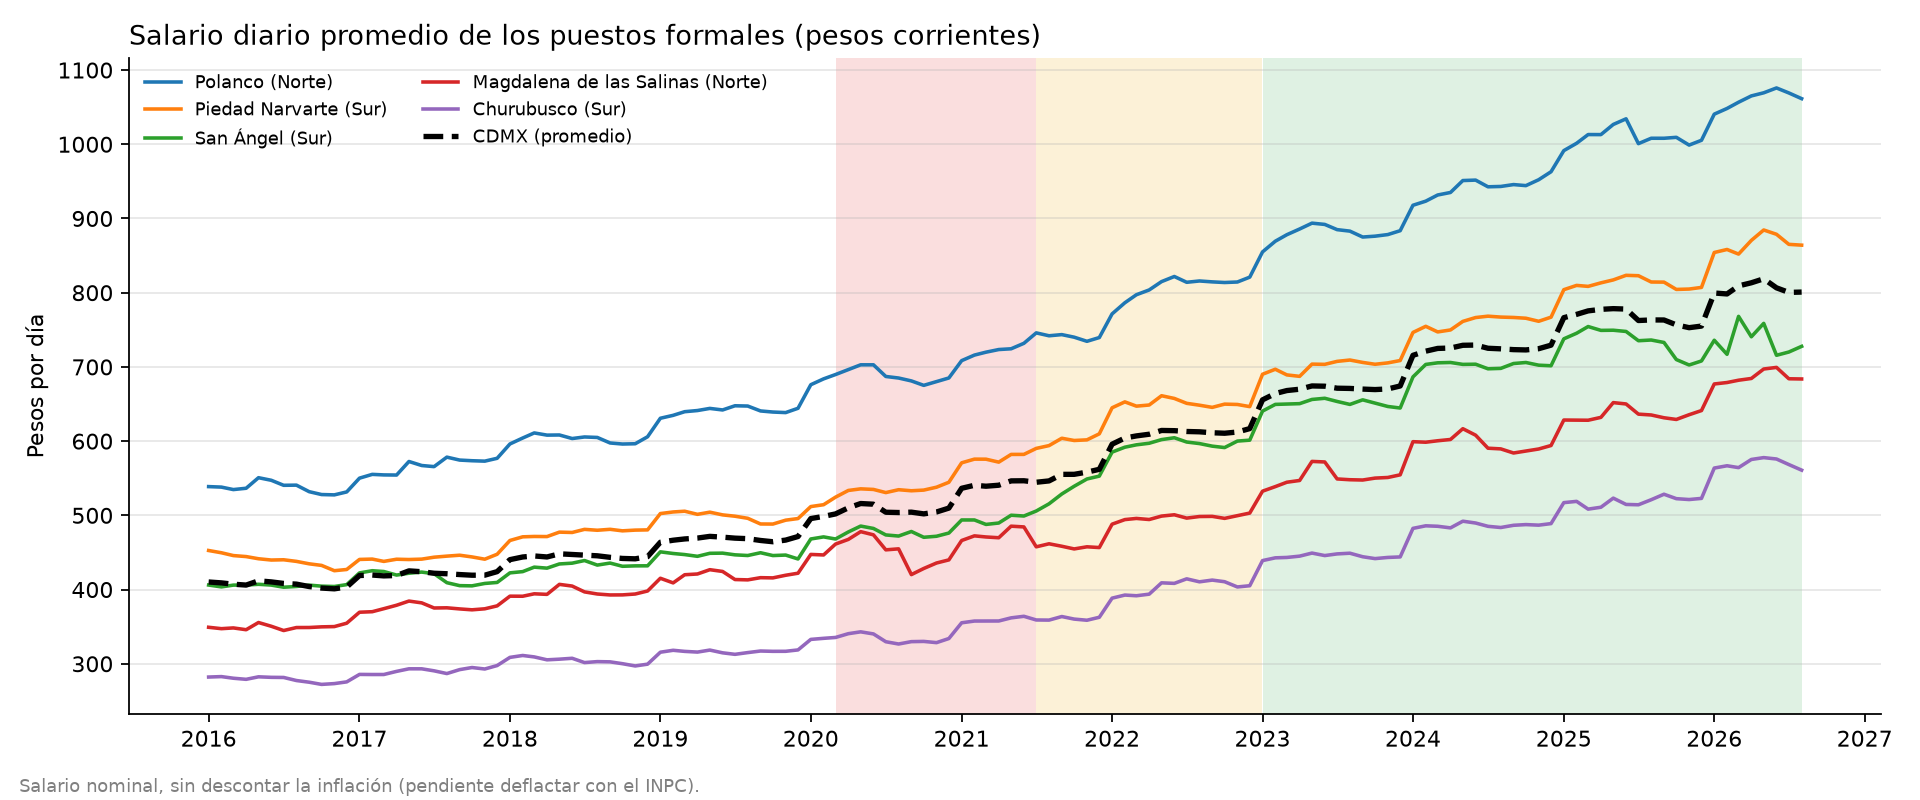
\includegraphics[width=\textwidth]{figuras/imss_salario_subdelegaciones.png}
\caption{Salario diario promedio (pesos corrientes) por subdelegación y promedio de la CDMX.}\label{fig:imss_salario}
\end{figure}

\subsection{Ocupación hotelera}
La serie mensual del porcentaje de ocupación hotelera (octubre de 2018 a julio de 2024) no tiene
vacíos, meses faltantes, duplicados ni valores fuera del rango 0--100\,\%. Los valores de abril a
junio de 2020 (1.6 a 3.4\,\%) son reales, porque corresponden al confinamiento, y se conservan. La
limpieza, hecha en el notebook 01, consistió en tres pasos:
\begin{enumerate}
  \item \textbf{Redondeo a dos decimales.} 47 de los 70 valores, entre febrero de 2020 y abril de
        2024, traían más de dos decimales. Los demás traían dos. Esto sugiere que la fuente cambió
        su forma de calcular el dato al inicio de la pandemia.
  \item \textbf{Fecha al primer día del mes,} en lugar del último, para poder unirla con las demás
        fuentes.
  \item \textbf{Nombre de columna} \archivo{ocupacion_pct}.
\end{enumerate}
El resultado se guardó en \archivo{data/interim/hoteles_mes.csv}. La ocupación promedio fue de
67.7\,\% en 2019. Bajó a 1.55\,\% en mayo de 2020 y en 2023 fue de 63.6\,\%, es decir, unos 4 puntos
por debajo del nivel previo a la pandemia. Queda pendiente estimar 2016 a septiembre de 2018 con
\emph{backcasting}, en el paso de completar (Figura~\ref{fig:hoteles}).

\begin{figure}[h]
\centering
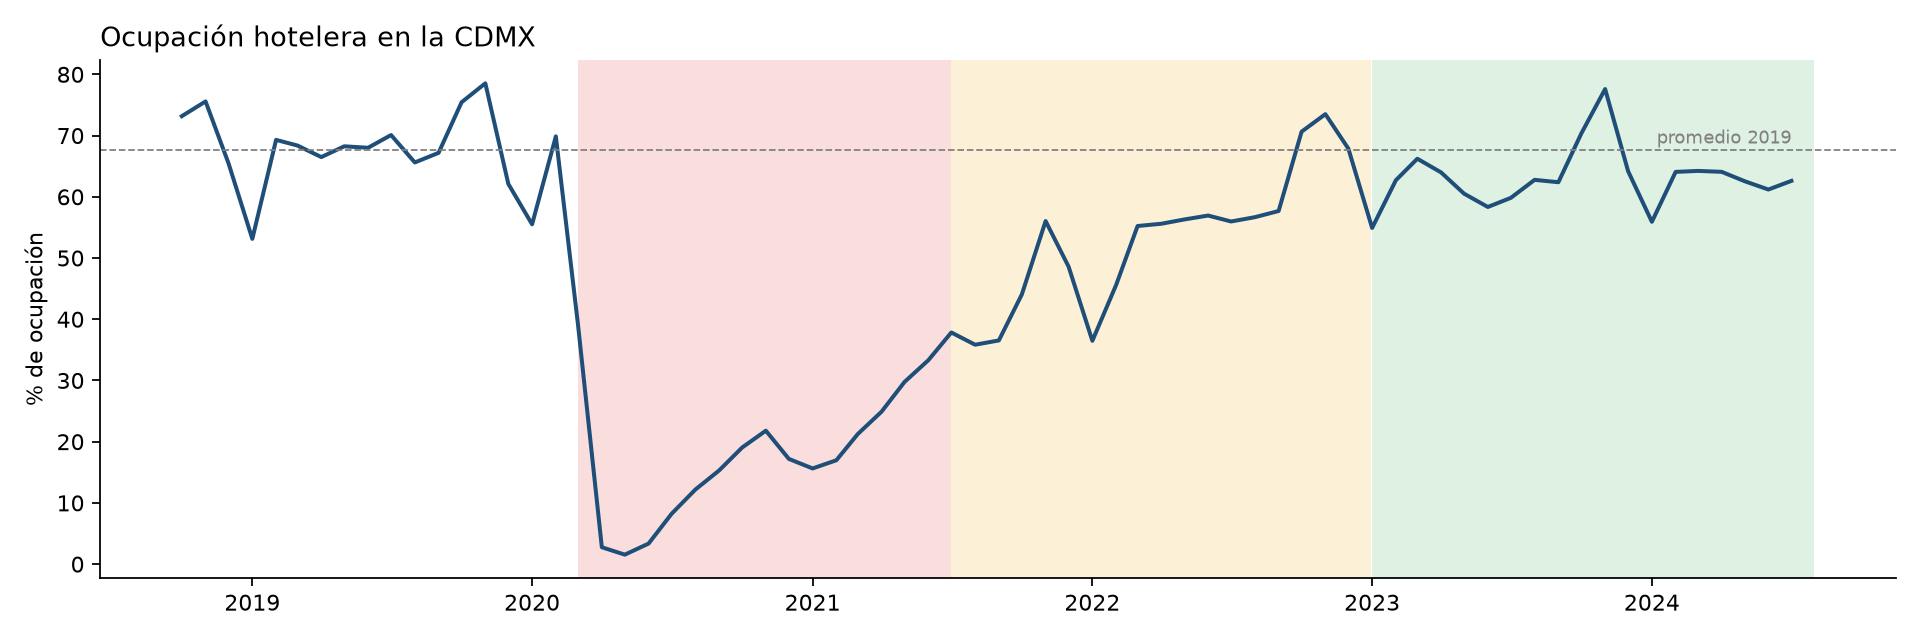
\includegraphics[width=\textwidth]{figuras/hoteles_ocupacion.png}
\caption{Ocupación hotelera mensual en la CDMX. La línea punteada es el promedio de 2019.}\label{fig:hoteles}
\end{figure}

\subsection{Hechos de tránsito}
Se unieron la serie ampliada (2018--2023) y la de 2024, y se construyó una tabla con el número de
accidentes por mes, alcaldía y tipo, junto con las personas lesionadas y fallecidas. Son 8,064 filas:
84 meses por 16 alcaldías por 6 tipos. Las combinaciones sin accidentes se registran como 0, porque no
son datos faltantes. El notebook 01 incluye al final de la sección una tabla con todos los errores
encontrados, los registros afectados y la decisión tomada. Los principales fueron:
\begin{itemize}
  \item \textbf{Formatos distintos} de fecha (aaaa-mm-dd frente a dd/mm/aaaa) y de hora entre los
        dos archivos.
  \item \textbf{Folio \enquote{SD}} (sin dato) en 7,288 registros, casi todos de 2018. Los folios
        repetidos corresponden a accidentes distintos, así que se contaron filas y no folios.
  \item \textbf{28 duplicados reales}, con la misma fecha, hora, tipo y coordenadas. Se eliminaron.
  \item \textbf{Nombres de alcaldía no estándar}, como \enquote{GUSTAVO A MADERO},
        \enquote{CUAJIMALPA} o la errata \enquote{CUAHUTEMOC}, y una avenida registrada como alcaldía
        (\enquote{AV INSURGENTES}). Se unificaron a la clave INEGI; la avenida se asignó por
        coordenadas.
  \item \textbf{El nombre de la alcaldía coincide con las coordenadas en el 95.8\,\% de los casos},
        frente al 99.7\,\% de la FGJ. Se conservó la alcaldía del registro. La diferencia
        probablemente se debe a accidentes en los límites entre alcaldías.
\end{itemize}

\begin{table}[h]
\centering
\caption{Hechos de tránsito por año (164,706 accidentes).}\label{tab:transito}
\small
\begin{tabular}{lrrrrr}
\toprule
\textbf{Año} & \textbf{Choque} & \textbf{Atropellado} & \textbf{Caída de ciclista} & \textbf{Total} & \textbf{Fallecidos}\\
\midrule
2018 & 9,608 & 4,297 & 156 & 17,025 & 394\\
2019 & 8,471 & 5,086 & 133 & 18,014 & 397\\
2020 & 9,251 & 2,761 & 544 & 16,440 & 388\\
2021 & 13,445 & 3,468 & 762 & 22,855 & 424\\
2022 & 18,523 & 4,676 & 845 & 30,702 & 533\\
2023 & 17,593 & 4,552 & 711 & 29,020 & 472\\
2024 & 18,109 & 4,821 & 760 & 30,650 & 533\\
\bottomrule
\end{tabular}
\end{table}

\paragraph{Tabla diaria.} Por si el análisis la requiere, se generó también
\archivo{transito_alcaldia_dia}, con los mismos accidentes por día, alcaldía y tipo: 245,472 filas
(2,557 días por 16 alcaldías por 6 tipos). Sus sumas coinciden mes por mes con la tabla mensual. No
falta ningún día, pero siete días tienen menos del 40\,\% de los registros normales según la mediana
móvil de 29 días. Por ejemplo, el 7 de mayo de 2018 tiene 4 accidentes y el 26 de junio de 2023 tiene
10, cuando lo normal es alrededor de 30 y 80. Probablemente son días con registro incompleto: se
conservan y se marcan con la columna \archivo{registro\_bajo}.

\paragraph{Problemas detectados al graficar.} Las gráficas revelaron dos cortes de registro que
no se veían en las tablas, y que se agregaron a la tabla de errores del notebook:
\begin{itemize}
  \item \textbf{Caídas de ciclista:} pasan de unas 11 a unas 65 al mes en \emph{febrero de 2020},
        antes del confinamiento. Un salto tan brusco y previo a la pandemia indica un cambio en la
        forma de registrar este tipo de accidente, no un aumento de ciclistas. Por eso no se usa para
        comparar antes y después.
  \item \textbf{Primer semestre de 2018:} los atropellados son la mitad que en el segundo semestre
        (unos 230 contra 450 al mes), y en 2018 el 43\,\% de los registros no tiene folio. El registro
        parece incompleto, así que la línea base de esta fuente es 2019.
\end{itemize}

\paragraph{Primeros resultados.} Los \textbf{atropellados} son el indicador más confiable de esta
fuente. Cayeron un 68\,\% en abril--mayo de 2020 (134 al mes, frente a 424 en 2019) y en 2024
volvieron al 95\,\% del nivel de 2019 (Figura~\ref{fig:transito_peatones}). Por alcaldía
(Figura~\ref{fig:transito_alcaldia}), la caída de 2020 fue mayor en las alcaldías centrales y de
oficinas que en las periféricas y populares:
\begin{itemize}
  \item Centrales: Coyoacán 38, Miguel Hidalgo 43, Cuauhtémoc 45 y Benito Juárez 48 (2019 = 100).
  \item Periféricas: Iztapalapa 63, Gustavo A.~Madero 68 e Iztacalco 68.
  \item Excepciones: Milpa Alta, periférica, cayó tanto como las centrales (43), y Venustiano
        Carranza, central, cayó poco (68). Milpa Alta tiene pocos atropellados al año, así que su
        índice varía mucho.
\end{itemize}
Esto es coherente con la hipótesis H4: donde más gente pudo trabajar desde casa, menos personas
salieron a la calle. Las muertes en hechos de tránsito se mantuvieron en unas 395 al año entre 2018 y
2020 y subieron hasta 533 en 2022 y 2024 (Figura~\ref{fig:transito_fallecidos}). El aumento se
concentra en los derrapados, típicamente de motocicleta (de 33 a 106), aunque parte puede deberse al
cambio de registro.

\begin{figure}[h]
\centering
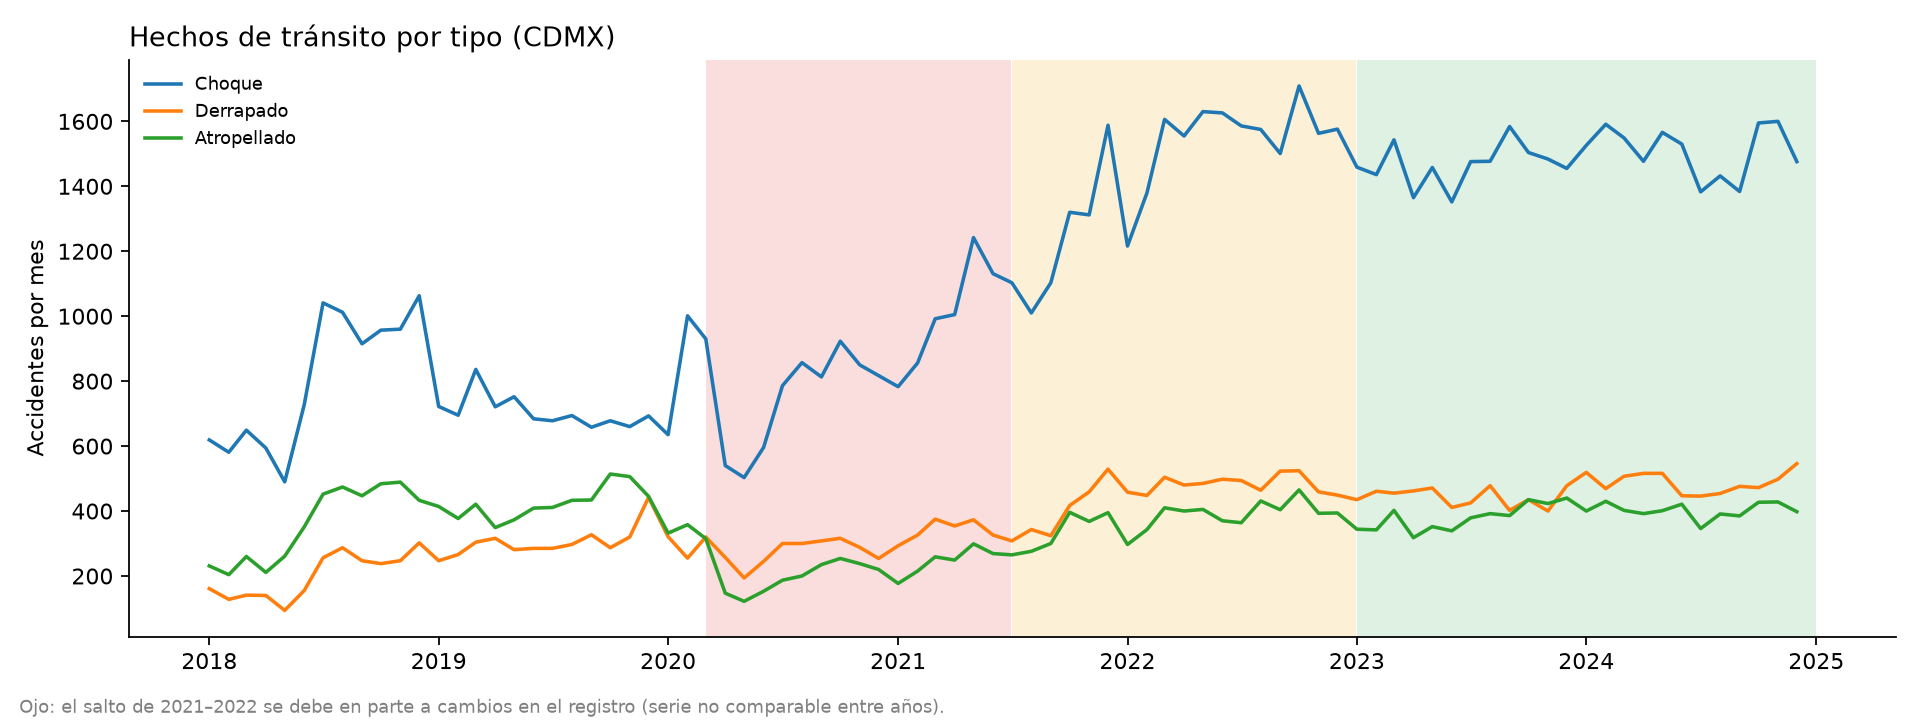
\includegraphics[width=\textwidth]{figuras/transito_tipos_mes.png}
\caption{Hechos de tránsito mensuales por tipo. El salto de 2021--2022 se debe en parte al cambio de registro.}\label{fig:transito_tipos}
\end{figure}

\begin{figure}[h]
\centering
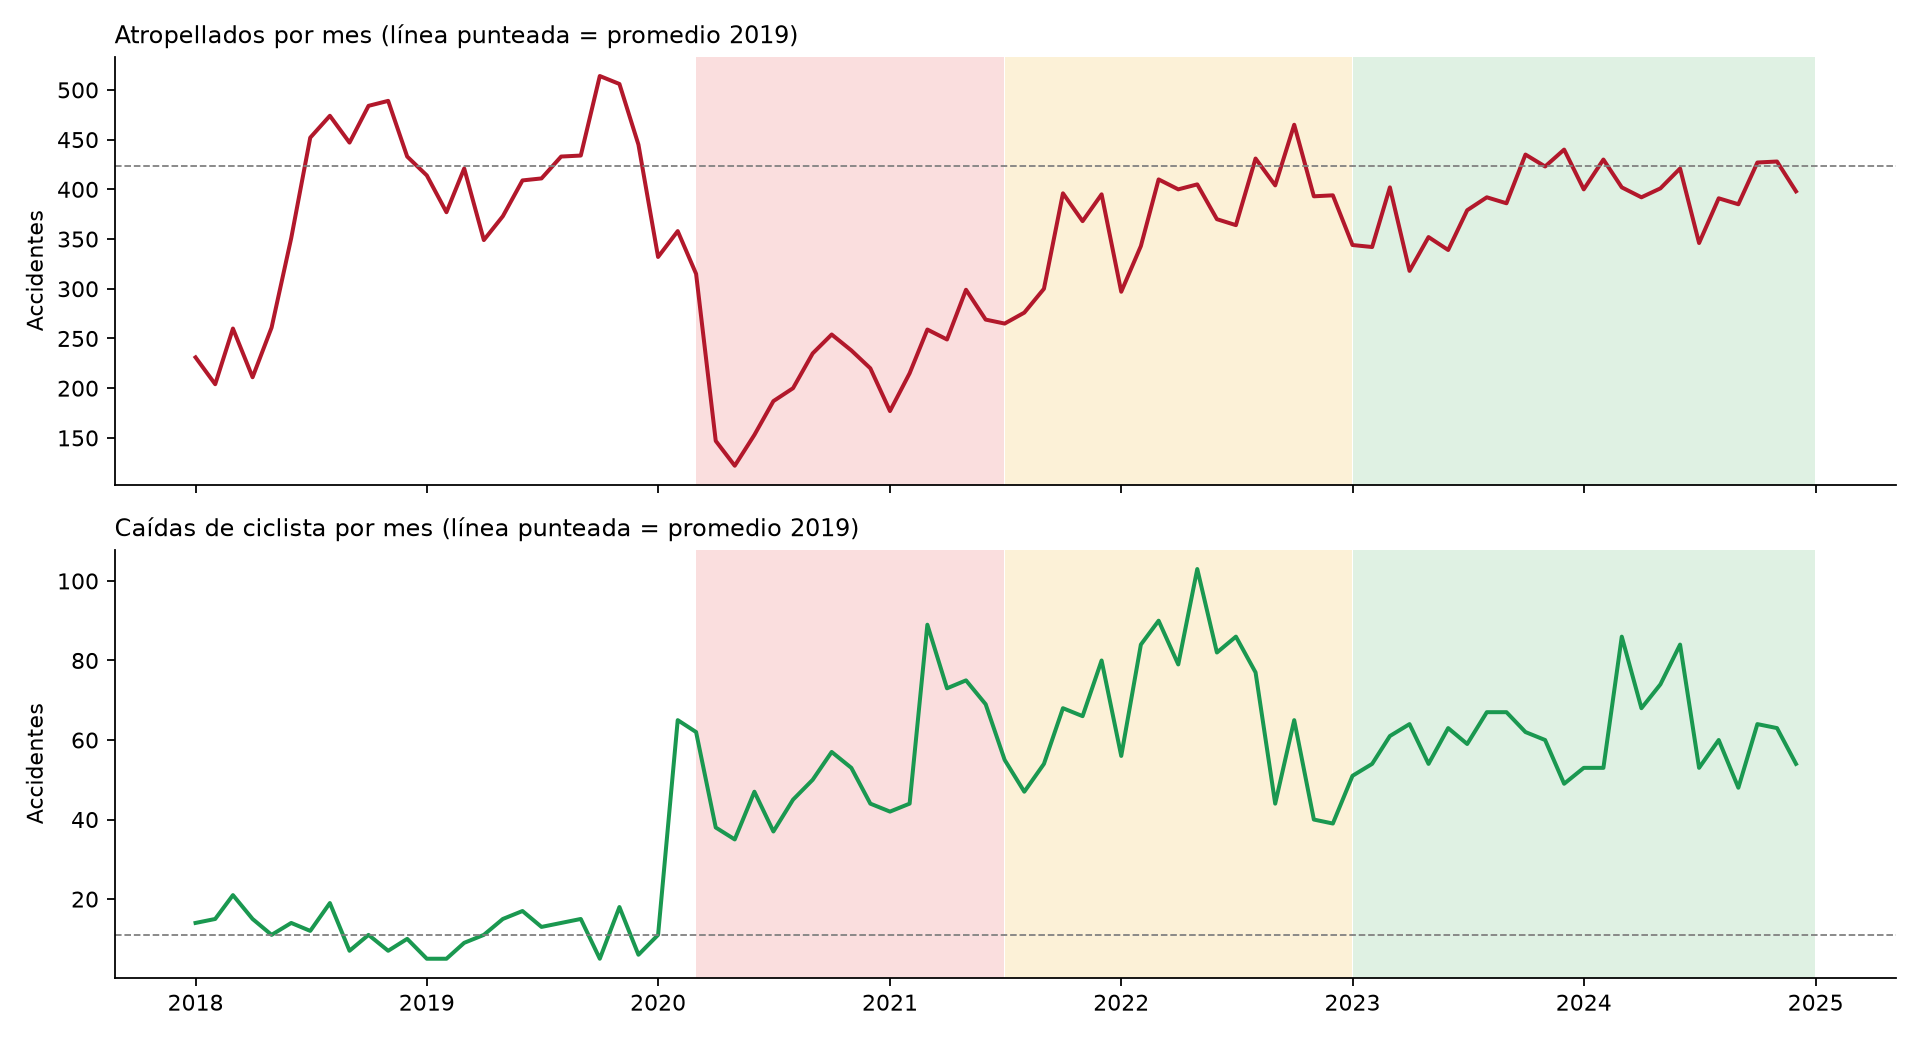
\includegraphics[width=\textwidth]{figuras/transito_peatones_ciclistas.png}
\caption{Atropellados y caídas de ciclista por mes. Obsérvese el corte de registro de febrero de 2020 en las caídas de ciclista.}\label{fig:transito_peatones}
\end{figure}

\begin{figure}[h]
\centering
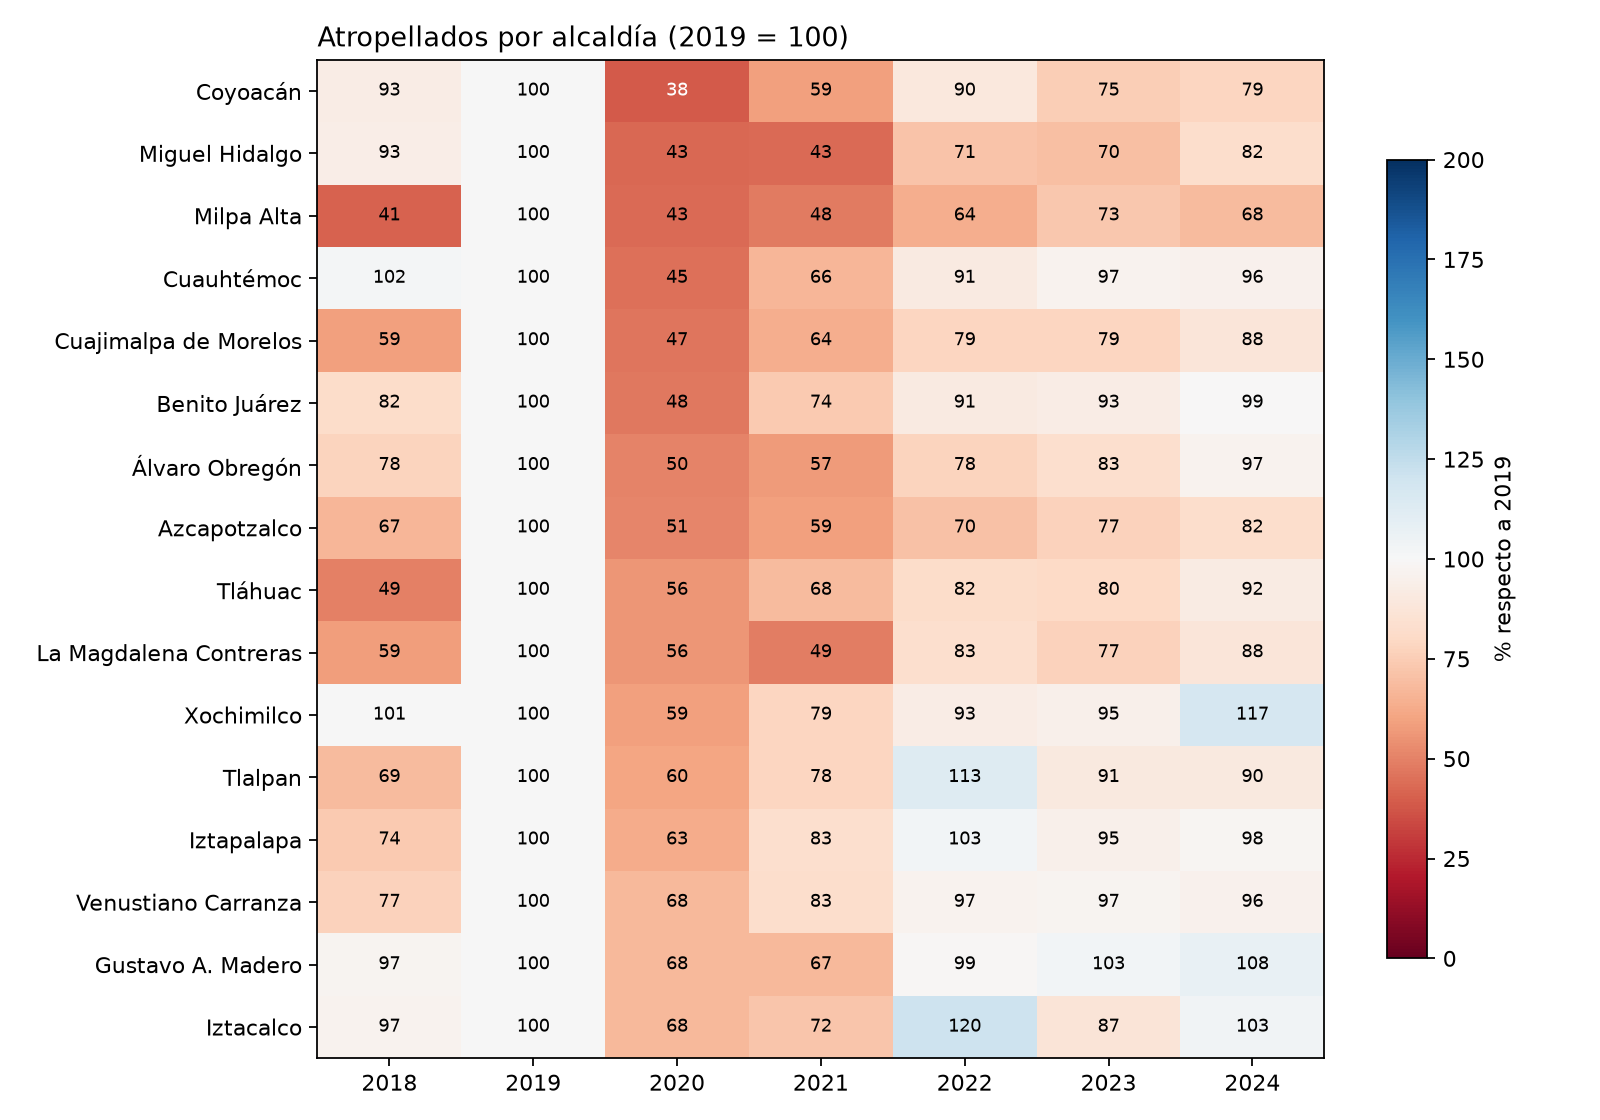
\includegraphics[width=.85\textwidth]{figuras/transito_atropellados_alcaldia.png}
\caption{Atropellados por alcaldía, índice 2019 = 100. Los valores de 2018 están subestimados por registro incompleto.}\label{fig:transito_alcaldia}
\end{figure}

\begin{figure}[h]
\centering
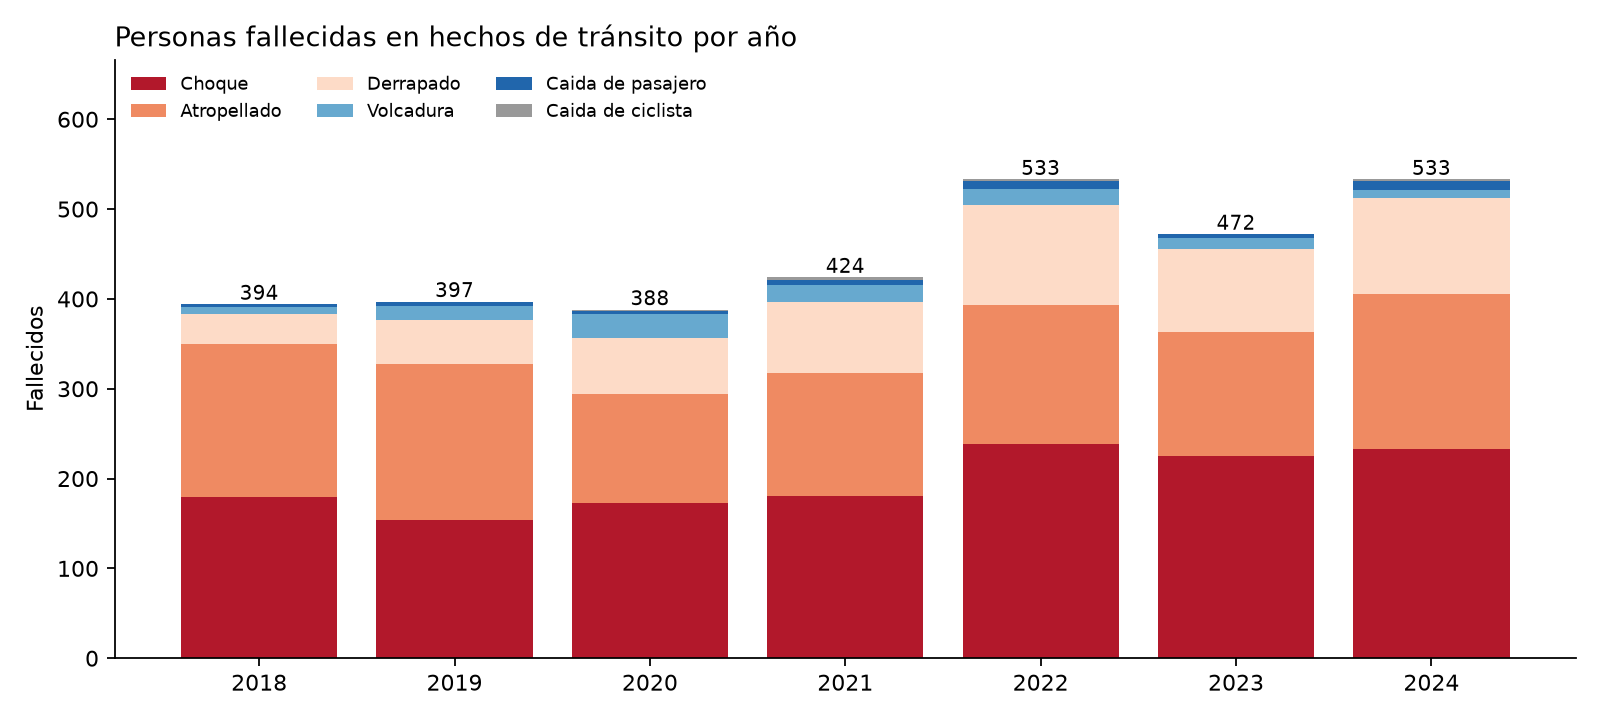
\includegraphics[width=.85\textwidth]{figuras/transito_fallecidos.png}
\caption{Personas fallecidas en hechos de tránsito por año y tipo de accidente.}\label{fig:transito_fallecidos}
\end{figure}

\subsection{Afluencia del Metro}
La limpieza se hizo por pasos en el notebook 01, a partir de \archivo{afluencia_metro_simple.csv}
(1,180,920 registros: 195 estaciones por día entre enero de 2010 y julio de 2026). La versión
desglosada por tipo de pago solo existe desde 2021 y suma exactamente lo mismo día por día, así que no
se usó. No hay celdas vacías, días faltantes ni valores negativos; los problemas estaban en los
nombres y en el significado de los ceros (Tabla~\ref{tab:limpieza_metro}).

\begin{table}[h]
\centering
\caption{Errores encontrados en la limpieza del Metro.}\label{tab:limpieza_metro}
\small
\begin{tabular}{L{7.2cm}rL{5cm}}
\toprule
\textbf{Error} & \textbf{Registros} & \textbf{Decisión}\\
\midrule
Línea escrita \archivo{Línea N} (2021--2023) y \archivo{Linea N} (resto) & 171,795 & Se repara y se unifica a \archivo{Línea N} (24 $\rightarrow$ 12)\\
Nombre de estación con \emph{mojibake} (\archivo{Católica}) & 379,245 & Se repara con \archivo{ftfy}\\
Gómez Farias / Peñón viejo (desde 2023-06) & 2,314 & Se unifican a la escritura anterior\\
Línea~B, dic-2020: \enquote{Oceanía} dos veces por día y falta \enquote{Deportivo Oceanía} & 31 & El 2.º registro se reasigna a Deportivo Oceanía\\
Ceros de la Línea~12 antes de su inauguración & 20,780 & Vacío; estado \archivo{no\_existia}\\
Sistema completo en $\approx$0 (servicio gratuito: 16--17 mar 2016 y 20--27 sep 2017) & 1,950 & Vacío; estado \archivo{sin\_registro}\\
Estación cerrada (COVID, obras de L1 y L12, incendio del PCC) & 39,667 & Es un 0 real; estado \archivo{cerrada}\\
Días $>$ 4 veces la mediana móvil de 29 días & 90 & Se conservan (12 de diciembre, conciertos, reaperturas)\\
\bottomrule
\end{tabular}
\end{table}

\paragraph{Duplicado de Oceanía.} En diciembre de 2020 la estación Oceanía de la Línea~B aparece dos
veces por día y Deportivo Oceanía no aparece. El primer registro promedia 5,307 viajes, parecido a
Oceanía en noviembre (5,625), y el segundo 7,054, parecido a Deportivo Oceanía (7,310). Además, el
segundo ocupa en el archivo el lugar de Deportivo Oceanía en el orden de la línea. Por eso se trató
como un error de etiqueta y se reasignó en lugar de borrarse.

\paragraph{Tres tipos de ceros.} Un cero puede significar que la estación no existía, que el Metro
funcionó sin contar pasajeros o que la estación estuvo cerrada. Solo el último es un cero real. Los
días sin conteo se detectaron porque el total de todo el sistema fue menor al 10\,\% de su mediana
móvil. Coinciden con el servicio gratuito posterior al sismo del 19-S y con la contingencia ambiental
de marzo de 2016. Se dejaron vacíos para no simular que nadie usó el Metro, y los promedios mensuales
se calculan solo con los días que tienen dato.

\paragraph{Salidas.} La tabla por estación y día supera el límite de filas de Excel, así que se
guardaron tres agregados en CSV y Parquet: \archivo{metro_linea_dia} (71,633 filas),
\archivo{metro_estacion_mes} (38,125) y \archivo{metro_mes} (199 meses, con el total, los días con
dato, las estaciones cerradas en promedio y una columna por línea). Los totales de las tres tablas
coinciden con los de la base depurada (23,155 millones de viajes).

\paragraph{Cierres de líneas.} La Línea~12 estuvo cerrada por completo desde el colapso del 3 de
mayo de 2021, reabrió por tramos desde enero de 2023 y por completo en enero de 2024. La Línea~1
cerró 12 estaciones por modernización desde julio de 2022 y reabrió por etapas hasta diciembre de 2025
(Figura~\ref{fig:metro_cierres}). Estos cierres quedan marcados en los datos para no confundirlos con
la falta de recuperación de la demanda.

\paragraph{Primeros resultados.} En mayo de 2020 la afluencia diaria fue el 26\,\% de la de 2019, y
el promedio de 2020 fue el 56\,\%, lo que apoya la hipótesis H1 (Figura~\ref{fig:metro_mensual}). En
2025 el Metro llegó al 79\,\% de 2019. Sin las Líneas~1 y 12 llega al 83\,\%: los cierres por obra
explican solo una parte de la diferencia y la demanda todavía no ha vuelto. La recuperación también
es desigual entre líneas (Figura~\ref{fig:metro_lineas}). En 2025 las Líneas~A, 9, 8, 12 y 4 están
entre 87 y 96, y las Líneas~2, 3, 5, 6, 7 y B entre 73 y 82. La Línea~1, todavía en obras
buena parte del año, llegó a 51.

\begin{figure}[h]
\centering
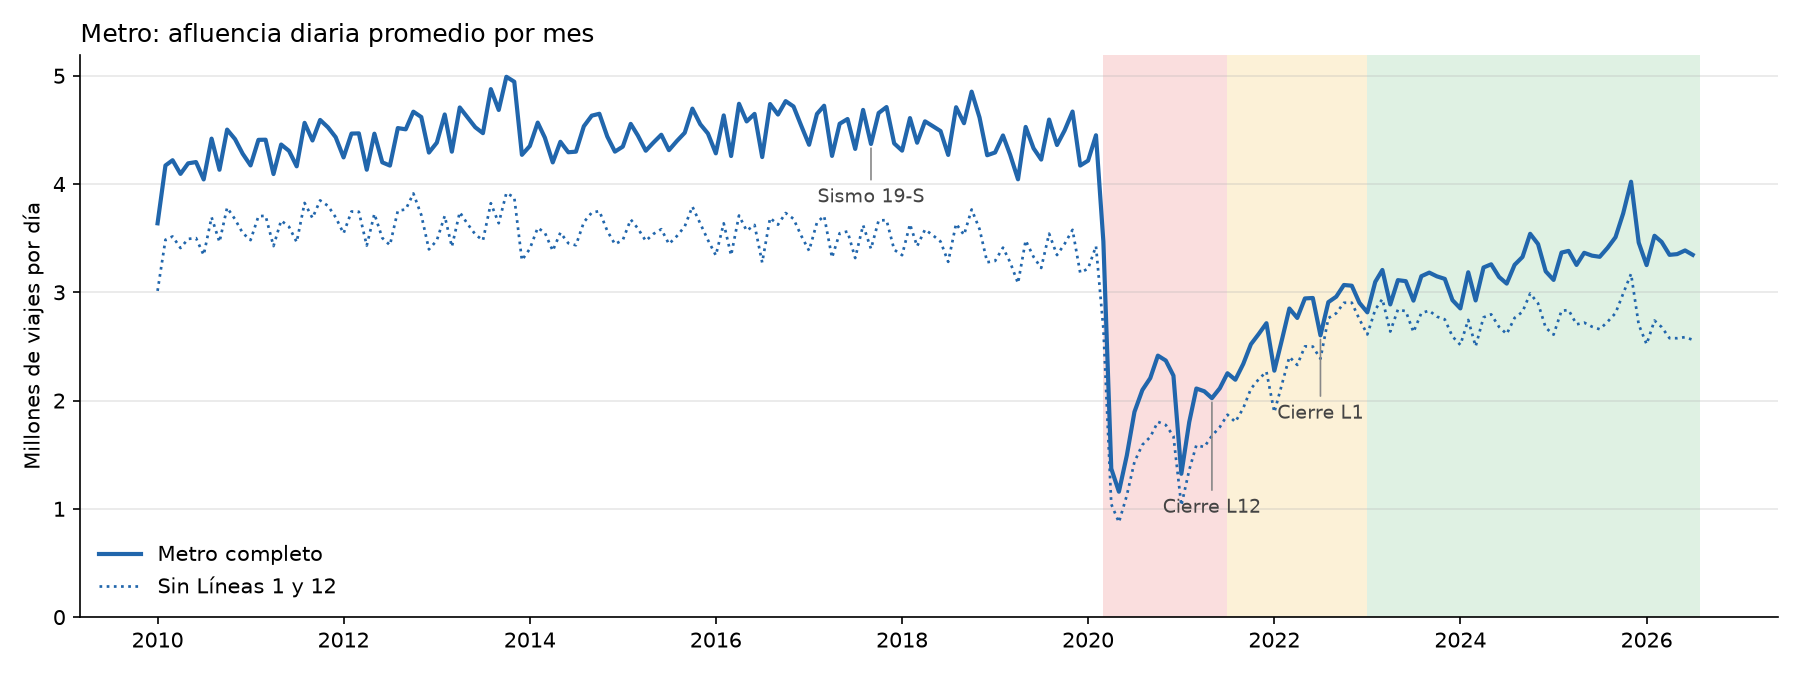
\includegraphics[width=\textwidth]{figuras/metro_limpio_mensual.png}
\caption{Afluencia diaria promedio mensual del Metro, completo y sin las Líneas~1 y 12. Las bandas marcan los periodos de choque, transición y post-pandemia.}\label{fig:metro_mensual}
\end{figure}

\begin{figure}[h]
\centering
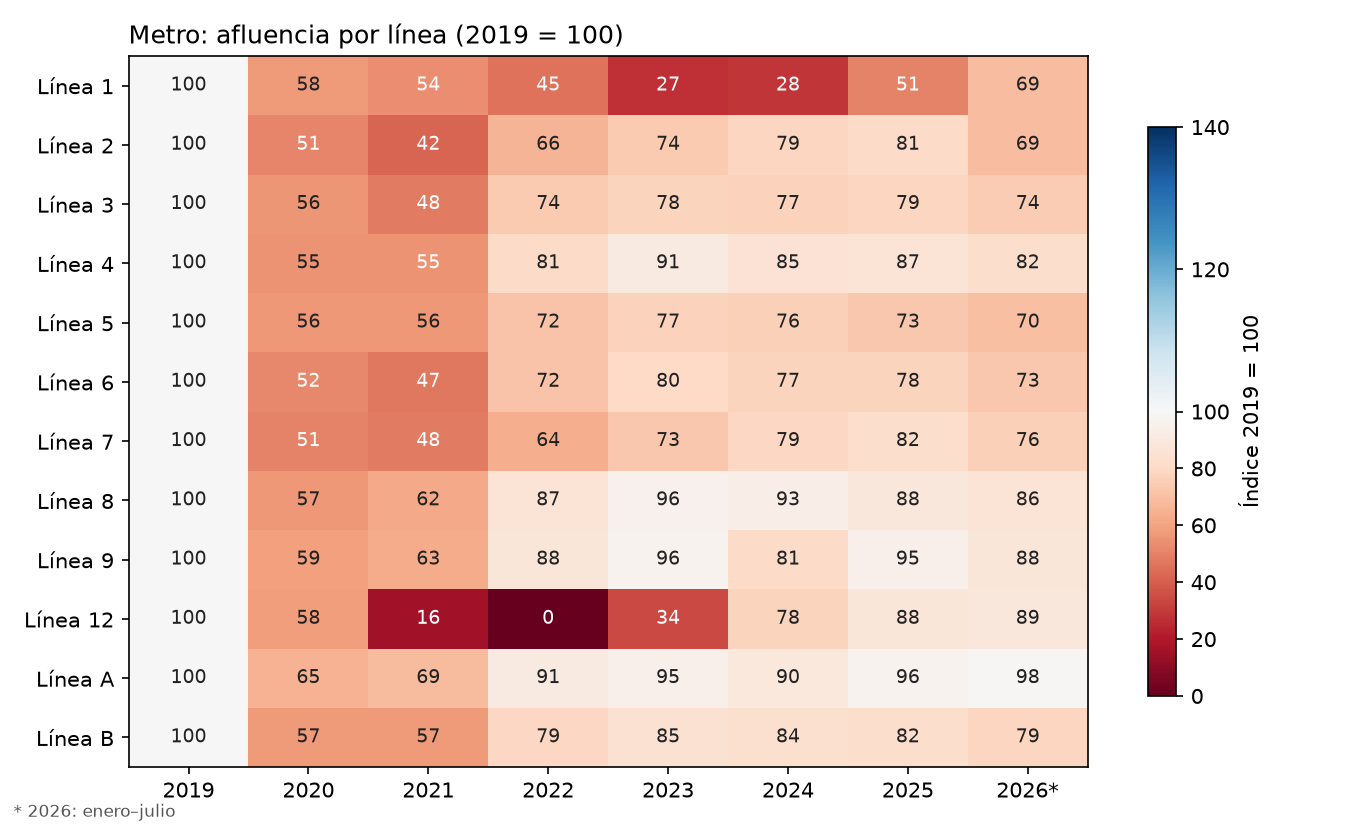
\includegraphics[width=.85\textwidth]{figuras/metro_lineas_indice.png}
\caption{Afluencia diaria promedio por línea y año, índice 2019 = 100.}\label{fig:metro_lineas}
\end{figure}

\begin{figure}[h]
\centering
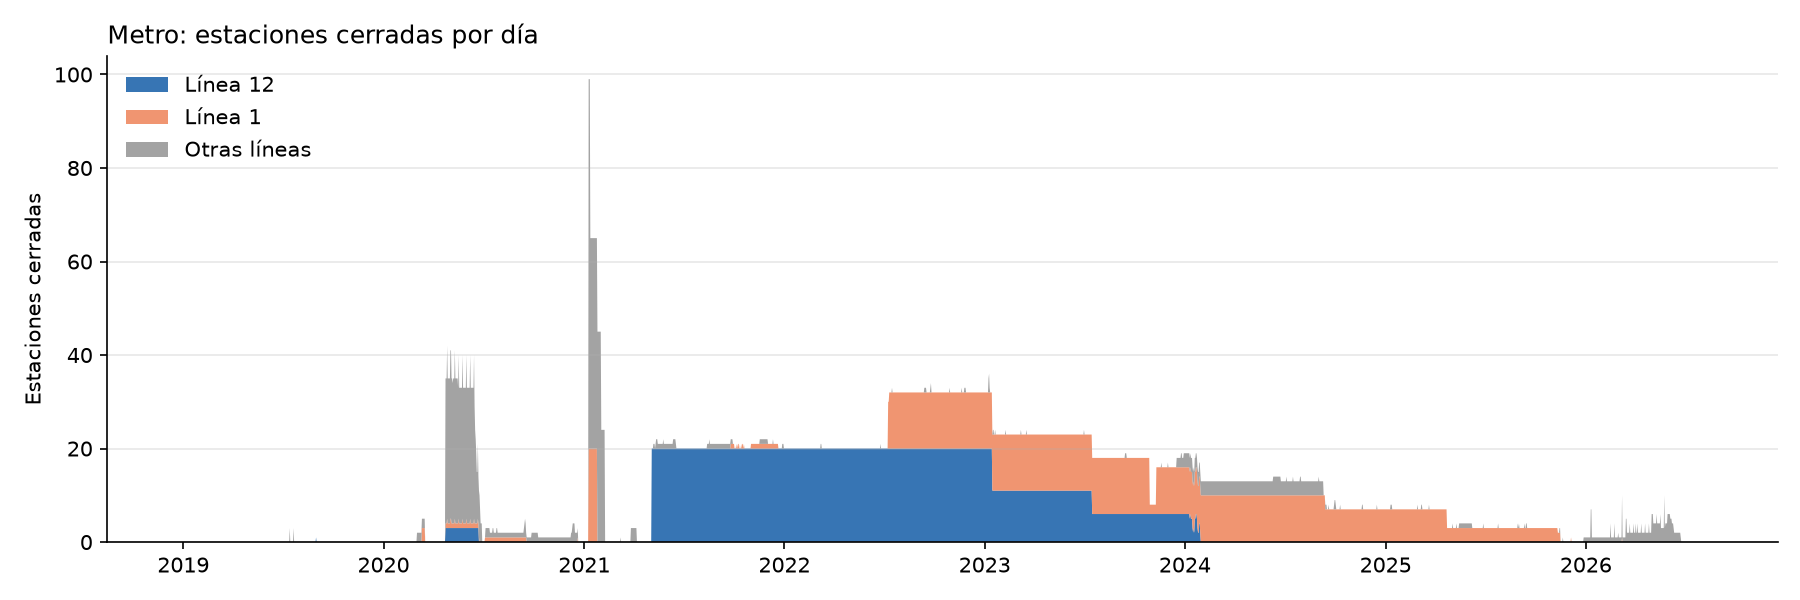
\includegraphics[width=\textwidth]{figuras/metro_cierres.png}
\caption{Estaciones del Metro cerradas por día. El pico de enero de 2021 corresponde al incendio del Puesto Central de Control.}\label{fig:metro_cierres}
\end{figure}

\subsection{Casos positivos de COVID-19}
Es la variable de control que mide la intensidad de la pandemia. El archivo tiene una fila por día
de toma de muestra entre el 5 de marzo de 2020 y el 8 de abril de 2023, con pruebas y positivos del
total de personas atendidas y de los residentes de la CDMX. Se usan los de residentes. No tiene
celdas vacías, y las tasas de positividad del archivo están bien calculadas. La limpieza se hizo en
el notebook 01 (Tabla~\ref{tab:limpieza_covid}).

\begin{table}[h]
\centering
\caption{Errores encontrados en la limpieza de los casos COVID.}\label{tab:limpieza_covid}
\small
\begin{tabular}{L{7.2cm}rL{5cm}}
\toprule
\textbf{Error} & \textbf{Registros} & \textbf{Decisión}\\
\midrule
Días de marzo de 2020 sin fila (sin muestras tomadas) & 17 & Se agregan con 0 y se marcan\\
Antes del 5-abr-2020, menos de 70 pruebas por día (arranque del registro) & 31 & Se conservan y se marcan\\
29-mar-2020: positivos de residentes (6) mayores que el total (5) & 1 & Se sube el total a 6\\
Fines de semana con muchas menos pruebas (el domingo, unas 4 veces menos que entre semana) & 323 & No es error: promedio móvil de 7 días y análisis semanal\\
\bottomrule
\end{tabular}
\end{table}

\paragraph{Salidas.} \archivo{covid_dia} (1,130 días), \archivo{covid_semana} (162 semanas, con la
misma semana ISO que el semáforo para poder unirlos) y \archivo{covid_mes} (38 meses). Las tasas
semanales y mensuales se calculan con las sumas del periodo, no como promedio de tasas diarias. La
primera y la última semana y el primer y el último mes están incompletos y se marcan. Después de
abril de 2023 no hay dato: al integrar se debe dejar vacío, no en 0.

\paragraph{Primeros resultados.} Se observan cuatro olas grandes (Figura~\ref{fig:covid}): la de
invierno 2020--2021 (unos 33 mil positivos por semana), Delta (23 mil), Ómicron, que es el máximo de
la serie con casi 60 mil en la tercera semana de 2022, y BA.5 a mitad de 2022 (46 mil). La
positividad llegó al 45\,\% a mitad de 2020, al 46\,\% con Ómicron y al 59\,\% con BA.5, así que
en esos momentos muchos contagios no se detectaban. Por eso, como control, conviene usar la tasa de
positividad junto con los positivos.

\begin{figure}[h]
\centering
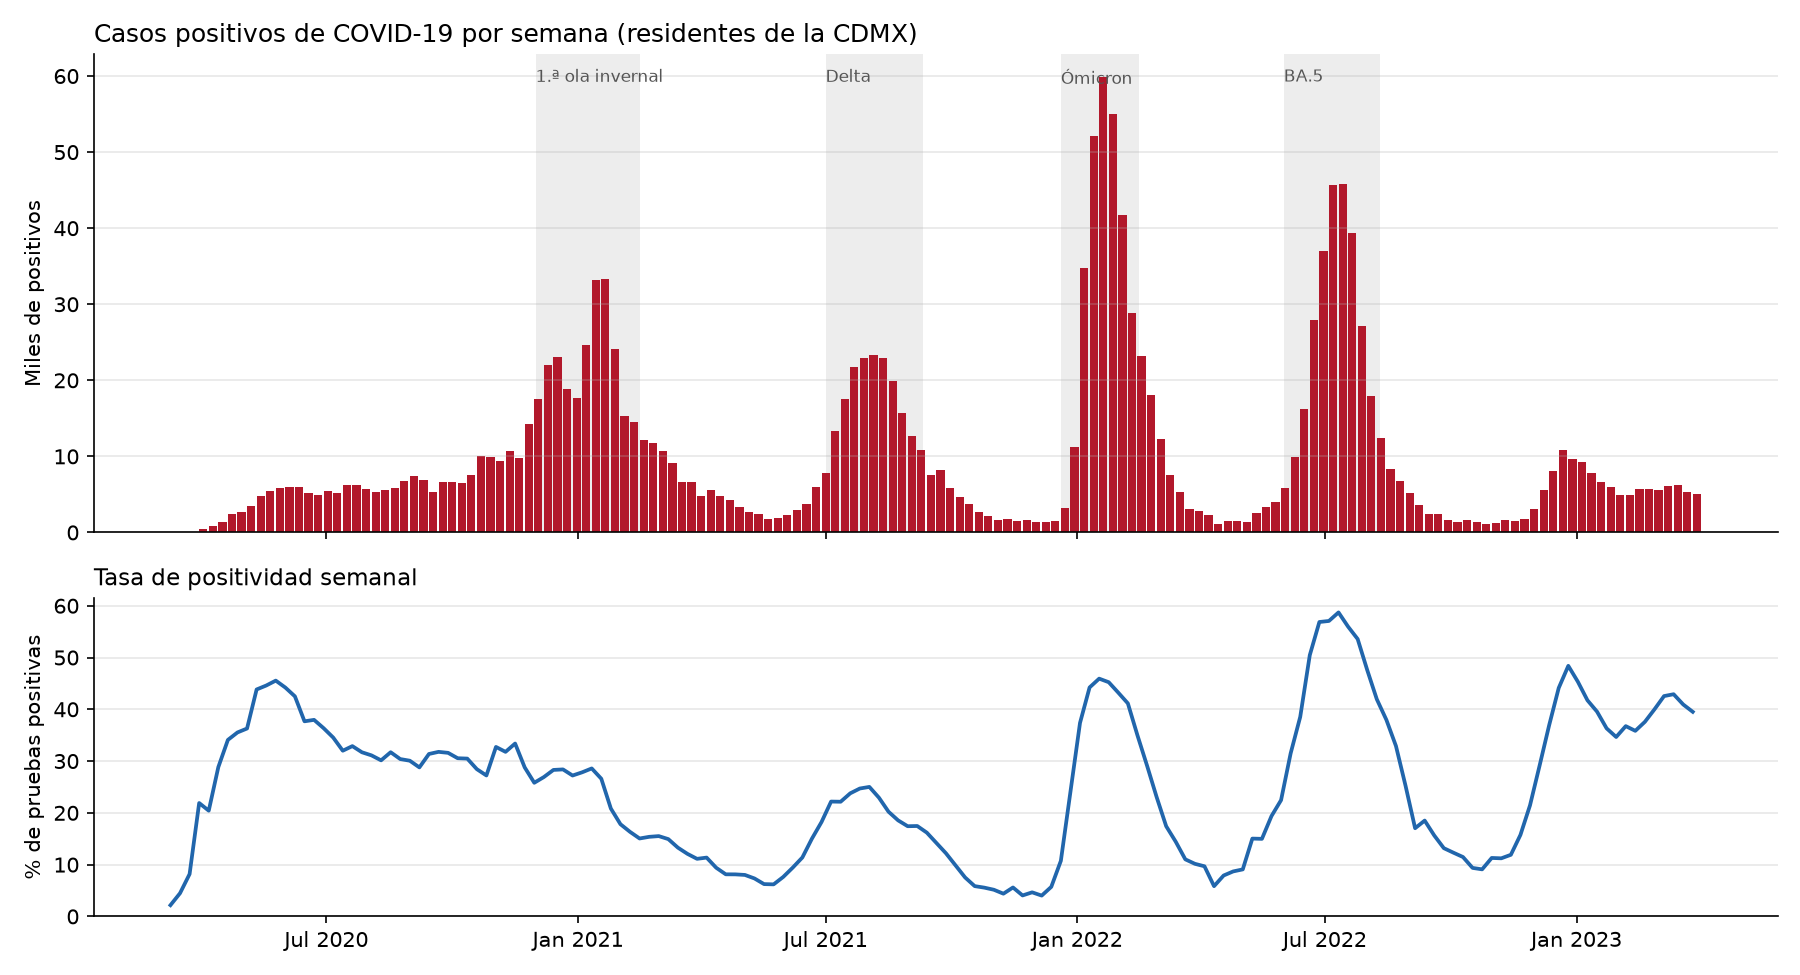
\includegraphics[width=\textwidth]{figuras/covid_semanal.png}
\caption{Casos positivos de COVID-19 por semana y tasa de positividad (residentes de la CDMX).}\label{fig:covid}
\end{figure}

\subsection{Semáforo epidemiológico}
Es la segunda variable de control: indica qué restricciones estaban vigentes cada semana. El archivo
viene en formato ancho, con una fila por entidad y una columna por semana ISO. La limpieza, hecha en el
notebook 01, consistió en cuatro pasos:
\begin{enumerate}
  \item \textbf{Filtrar la CDMX} y pasar a formato largo, con una fila por semana.
  \item \textbf{Fecha de la semana:} el lunes de cada semana ISO, igual que en \archivo{covid_semana},
        para poder unir las dos fuentes.
  \item \textbf{Semanas faltantes.} La revisión con \archivo{isna()} no encontró vacíos, pero al
        comparar contra el calendario completo faltaban dos semanas: 2020-W53 (2020 tuvo 53 semanas
        ISO) y 2022-W01.
  \item \textbf{Relleno.} En ambos casos la semana anterior y la siguiente tienen el mismo color (rojo
        y verde, respectivamente), así que se rellenaron con ese color y se marcaron con la columna
        \archivo{imputado}. Si los colores vecinos hubieran sido distintos, no se habría rellenado.
\end{enumerate}
El resultado, \archivo{semaforo_cdmx_semana.csv}, tiene 160 semanas, de 2020-W22 a 2023-W24: 15 en
rojo, 42 en naranja, 20 en amarillo y 83 en verde.
